%!TEX program = xelatex
% 完整编译: xelatex -> bibtex -> xelatex -> xelatex

\documentclass[lang=cn,11pt,a4paper]{elegantpaper}
\usepackage{mathtools}
\usepackage{minted}
\hypersetup{colorlinks=false} 
\usepackage{color}
\title{Match-Us 项目合作}
\author{}
\institute{}

\version{}
\date{\zhtoday}

\begin{document}

\maketitle

%\tableofcontents


\section{最佳匹配稳定性}

匹配稳定性是指,在一个匹配方案中,不存在这样一对匹配,其中一方在对方的偏好排序中不是第一位。

\begin{figure}[htb]
    \centering
    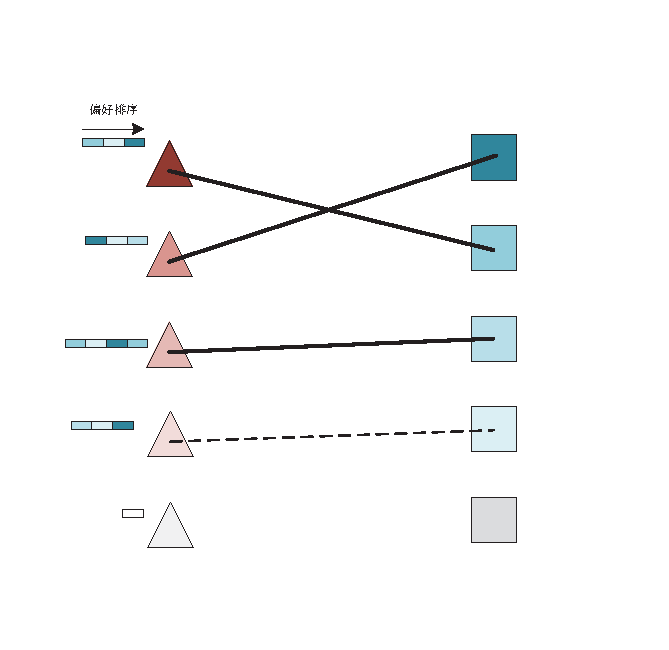
\includegraphics[scale=1]{favor.eps}
    \caption{最佳稳定性示例}
    \label{fig:my_label}
\end{figure}

关于满意度和匹配基数都可以被纳入到最佳稳定性的框架中。

\section{硬性、软性要求}

个人偏好排序列表: 偏序集 $F(i)$,$C(j)$。

\subsection{硬性要求}

硬性要求:性别,年龄,地区(?)......

根据硬性要求筛选。

\subsection{软性要求}

软性要求:性格,爱好......

根据软性要求打分排序。

\section{模型}

MAX-SMIT是$\mathcal{NP}$问题,需要整数规划建模求精确解。

\begin{equation}
\begin{aligned}
\max & \sum_{i=1}^{n_{1}} \sum_{j \in F(i)} x_{i j} \\
s.t. &\sum_{j \in F(i)} x_{i j} \leq 1, \quad i=1, \ldots, n_{1},\\
&\sum_{i \in C(j)} x_{i j} \leq 1, \quad j=1, \ldots, n_{2}, \\
&1-\sum_{q \in F_{j}^{\leq}(i)} x_{i q} \leq \sum_{p \in C_{i}^{s}(j)} x_{p j}, \quad i=1, \ldots, n_{1}, j \in F(i) \\
&x_{i j} \in\{0,1\}, \quad i=1, \ldots, n_{1}, j \in F(i)
\end{aligned}
\end{equation}

\section{其他}

\subsection{数据处理}

旧有的已配对数据(打分函数,假设检验)。

现有的几类数据建模归类。

\subsection{目标函数}

加入权重

$$\max & \sum_{i=1}^{n_{1}} \sum_{j \in F(i)} w(i,j) x_{i j} $$

\end{document}